%%%%%%%%%%%%%%%%%%%%%%%%%%%%%%%%%%%%%%%%%%%%%%%%%%%%%%%%%%%%%%%%%%%%%%%%%%%%%%%%
\section{Shape-from-Shading}\label{sec:bg_sfs}
%%%%%%%%%%%%%%%%%%%%%%%%%%%%%%%%%%%%%%%%%%%%%%%%%%%%%%%%%%%%%%%%%%%%%%%%%%%%%%%%
%%%%%%%%%%%%%%%%%%%%%%%%%%%%%%%%%%%%%%%%
\begin{figure*}[t]
	\centering
	\begin{subfigure}[b]{0.24\textwidth}
		\centering
		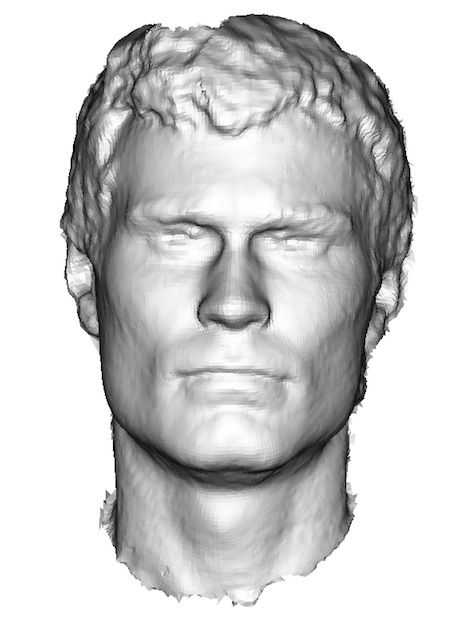
\includegraphics[height=2in]{background/images/frontal}
		\caption*{Frontal}
	\end{subfigure}
	\begin{subfigure}[b]{0.24\textwidth}
		\centering
		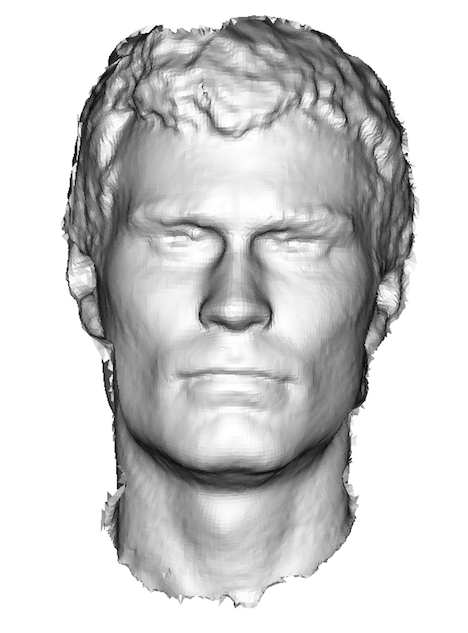
\includegraphics[height=2in]{background/images/invert}
		\caption*{Inverted}
	\end{subfigure}
	\begin{subfigure}[b]{0.24\textwidth}
		\centering
		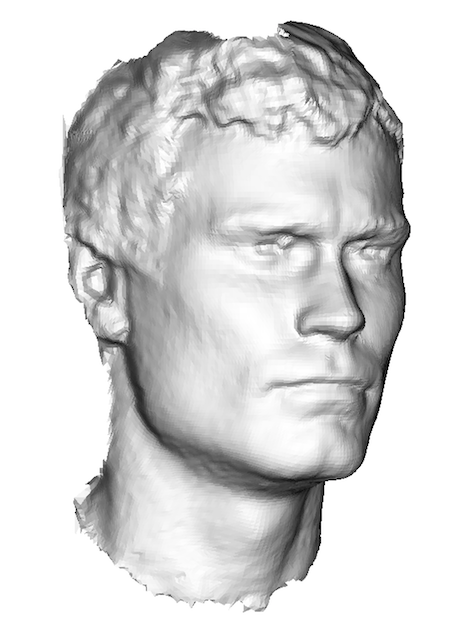
\includegraphics[height=2in]{background/images/frontal_rotate}
		\caption*{Frontal}
	\end{subfigure}
	\begin{subfigure}[b]{0.24\textwidth}
		\centering
		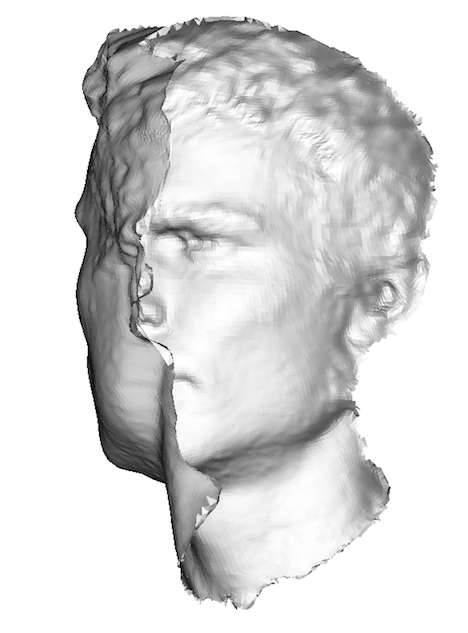
\includegraphics[height=2in]{background/images/invert_rotate}
		\caption*{Inverted}
	\end{subfigure}
	\caption{An example of a bas-relief ambiguity for a mesh illuminated
	         frontally under orthographic projection, with a lambertian shader.
	         ``Inverted'' implies that the mesh is actually facing away from the
	         camera and thus the interior is visible, as demonstrated by the
	         rotated ``Inverted'' image. Both of the non-frontal images are
	         rotated versions of the frontal images, approximately $25^\circ$
	         around the Yaw axis.}
\label{fig:bg_sfs_bas_relief}
\end{figure*}
%%%%%%%%%%%%%%%%%%%%%%%%%%%%%%%%%%%%%%%%
Shape-from-shading (SfS)~\cite{horn1970shape} is the process of attempting to
recover surface information from an object in an image using \textit{inverse
rendering}, or \textit{image formation}, methods. The primary assumption is that
shading, or the intensity of a pixel in the image, is generated as a function of
the surface geometry and its interaction with light reflected/absorbed by the
surface and captured by an imaging device. Naturally, the reality of this
process in the physical world is a complex interaction between light and both
microscopic and macroscopic elements of the surface structure. This is further
complicated by the noise present in the recording procedure of the camera
sensing hardware. Furthermore, it is well known that shading alone is
insufficient to disambiguate shape. For example, the well known bas-relief
ambiguity~\cite{belhumeur1999bas} is demonstrated for a facial mesh in
\cref{fig:bg_sfs_bas_relief}. The bas-relief ambiguity states that for an object
imaged under orthographic projection that exhibits Lambertian reflectance, there
exists a family of transformations (generalized bas-relief transformations) for
which the images produced will be identical. In fact, more generally there
exists an infinite number of ways to describe any image given only shading
information through different arrangements of surfaces, lightings and
albedos~\cite{adelson1996perception}. However, despite the ill-posedness of the
SfS problem, shading does in fact provide a very strong imaging prior and many
higher frequency detail such as wrinkles can only be recovered using shading
cues. Before discussing the facial surface recovery literature, we briefly
describe the image formation problem including the common assumptions
made.
%%%%%%%%%%%%%%%%%%%%%%%%%%%%%%%%%%%%%%%%%%%%%%%%%%%%%%%%%%%%%%%%%%%%%%%%%%%%%%%%
\subsection{Image Formation}
%%%%%%%%%%%%%%%%%%%%%%%%%%%%%%%%%%%%%%%%%%%%%%%%%%%%%%%%%%%%%%%%%%%%%%%%%%%%%%%%
%%%%%%%%%%%%%%%%%%%%%%%%%%%%%%%%%%%%%%%%
\begin{figure*}[t]
	\centering
	\begin{tabular}{cc}
		\multicolumn{2}{c}{
			\begin{subfigure}[b]{\textwidth}
				\centering
				\caption*{Radiometric Terms}
				\begin{tabular}{@{}lll@{}}
					\toprule
					Term              & Symbol                                      & Unit                 \\ \midrule
					Solid Angle       & $d\omega$                                    & ${sr}^{-1}$          \\
					Radiant Flux      & $\Phi$                                       & $W$                  \\
					Radiant Intensity & $J = d \Phi / d \omega$                      & $W {sr}^{-1}$        \\
					Irradiance        & $E = d \Phi / d A$                           & $W m^{-2}$           \\
					Radiance          & $L = d^2 \Phi / (dA \cos{\theta_r} d\omega)$ & $W m^{-2} {sr}^{-1}$ \\ \bottomrule
				\end{tabular}
			\end{subfigure}
		} \\[2cm]
		\begin{subfigure}[b]{0.48\textwidth}
			\centering
			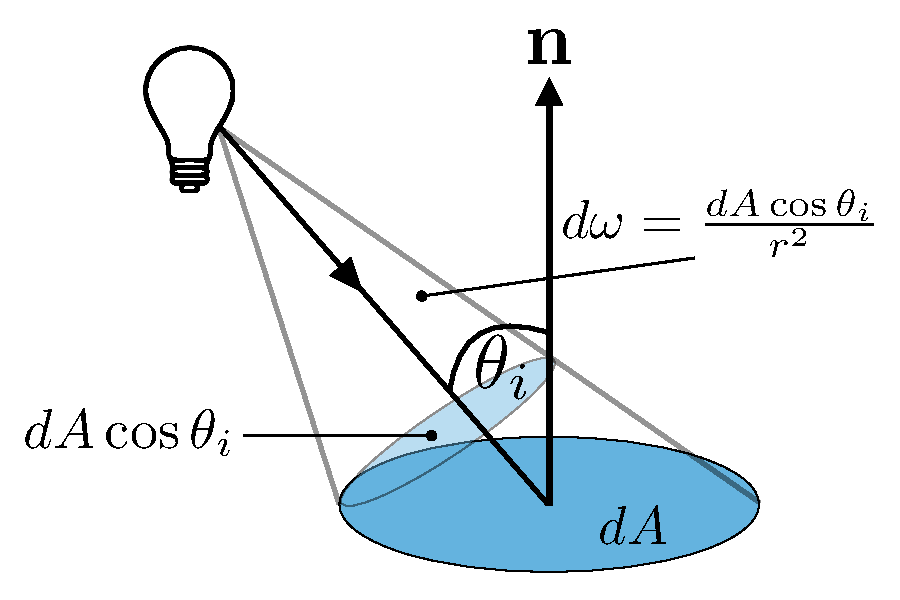
\includegraphics[width=\textwidth]{background/images/irradiance}
			\caption*{Irradiance}
		\end{subfigure} &
		\begin{subfigure}[b]{0.48\textwidth}
			\centering
			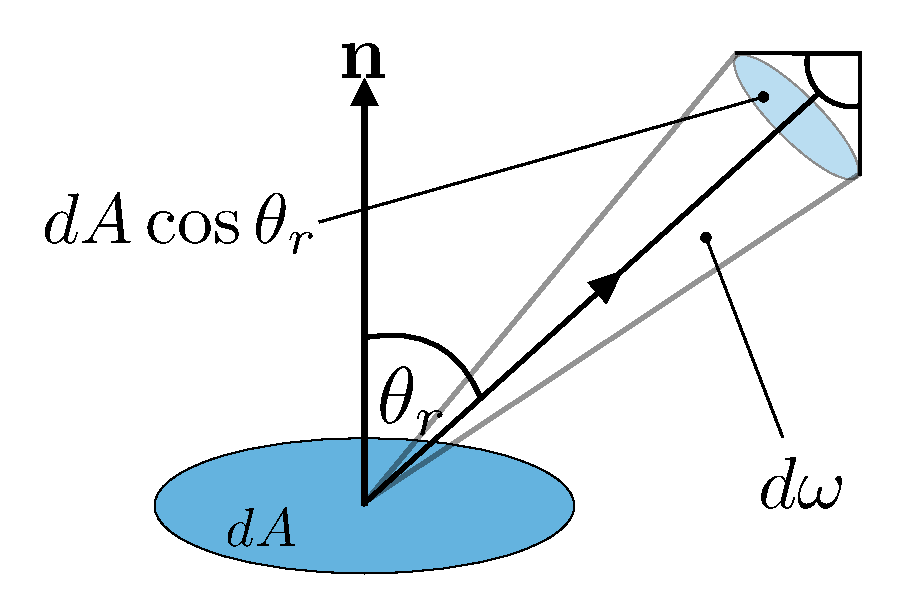
\includegraphics[width=\textwidth]{background/images/radiance}
			\caption*{Radiance}
		\end{subfigure}
	\end{tabular}
	\caption{Illustration of common radiometric terms, focusing on the surface
	         irradiance and radiance. ${sr}^{-1}$ denotes steradians, the
	         Standard International unit of solid angular measure and
	         $W$ denotes watts.}
\label{fig:bg_sfs_rad_irrad}
\end{figure*}
%%%%%%%%%%%%%%%%%%%%%%%%%%%%%%%%%%%%%%%%
%TODO: Need a section on Spherical Harmonics
When discussing image formation methods a number of assumptions are commonly
made in order to ensure tractability of the rendering physics. Firstly,
unless explicitly mentioned, we assume an orthographic camera projection. This
is a reasonable assumption for most facial images as faces tend to the be
the focus of an image and thus photographs are commonly taken close enough
to the face that perspective effects are minimal. We also only consider
reflection functions that can be expressed as a Bidirectional
Reflectance-Distribution Function (BRDF). A BRDF is a convenient construct
that allows the expression of how bright a surface will appear from a given
view point direction when illuminated from another direction. More formally, it
is the ratio of the reflected radiance in the viewing direction to the
irradiance, in the direction toward the light source.
See \cref{fig:bg_sfs_rad_irrad} for an illustration of the radiance and
irradiance as well as a table of useful radiometric terms. BRDFs are functions
of local illumination and do not model global illumination effects such
as shadows or inter-reflections.
\textit{Radiant flux} is the power emitted from a light source, measured in
watts $(W)$.
The \textit{solid angle} subtended by a surface patch is defined as the
surface area of a unit sphere covered by the surface's projection onto the
sphere and is measured in steradians $(sr)$. In \cref{fig:bg_sfs_rad_irrad},
$r$ refers to the distance from the sphere's origin to the patch.
\textit{Radiant intensity} is the radiant flux per unit solid angle and is
measured in watts per steradian $(W {sr}^{-1})$.
The \textit{irradiance} is the amount of energy received by a given surface
patch, measured in watts per square meter $(W m^{-2})$.
The \textit{radiance} is the amount of energy emitted per unit foreshortened
surface area per unit solid angle, measured in watts per square meter
per steradian $(W m^{-2} {sr}^{-1})$. In \cref{fig:bg_sfs_rad_irrad},
the unit foreshortened area is given by $dA \cos{\theta_r}$.
It is important to note that radiance, unlike irradiance, is a directional
quantity. This implies that the viewing angle affects the amount of perceived
light from a given image area and for some reflectance functions that manifests
as specular style highlights. Finally, we rely on the fact that the image
irradiance captured by the camera sensor is directly proportional to the
scene radiance~\cite{horn1979calculating}. To simplify matters, when referring
to image irradiance we assume that the linear relationship between the scene
radiance and image irradiance is the identity
\ie~scene radiance = image irradiance. An illustration of the relationship
between scene radiance and image irradiance is given in
\cref{fig:bg_sfs_scene_to_intensity}.

Given the previous definitions, we can now formally define the general equation
for a BRDF
%%%%%%%%%%%%%%%%%%%
\begin{align}\label{eg:bg_sfs_general_brdf}
	f(\theta_i,\phi_i;\theta_r,\phi_r) &= \frac{L(\theta_r,\phi_r)}{E(\theta_i,\phi_i)} \\
	L(\theta_r,\phi_r)                 &= E(\theta_i,\phi_i) f(\theta_i,\phi_i;\theta_r,\phi_r) \\
	L(\theta_r,\phi_r)                 &= \int_{2\pi} I_{\operatorname{src}}(\theta_i,\phi_i) f(\theta_i,\phi_i;\theta_r,\phi_r) \; \cos{\theta_i} \; d\omega_i,
\end{align}
%%%%%%%%%%%%%%%%%%%
where $I_{\operatorname{src}}(\theta_i,\phi_i)$ is the intensity of output
from a given light source. In fact, assuming isotropy, the BRDF is
only a function of 3 parameters, $f(\theta_i,\theta_r, \Delta \phi)$ where
$\Delta \phi = \phi_i - \phi_r$. An isotropic BRDF is invariant to rotations
around the direction of the normal. We also assume Helmholtz reciprocity, which
states that if the light source and viewing direction are swapped the BRDF
remains unchanged
\ie~$f(\theta_i,\phi_i;\theta_r,\phi_r) = f(\theta_r,\phi_r;\theta_i,\phi_i)$.
An illustration of the general BRDF is given in \cref{fig:bg_sfs_brdf_example}.
%%%%%%%%%%%%%%%%%%%%%%%%%%%%%%%%%%%%%%%%
\begin{figure*}[t]
	\centering
	\begin{subfigure}[b]{0.45\textwidth}
		\centering
		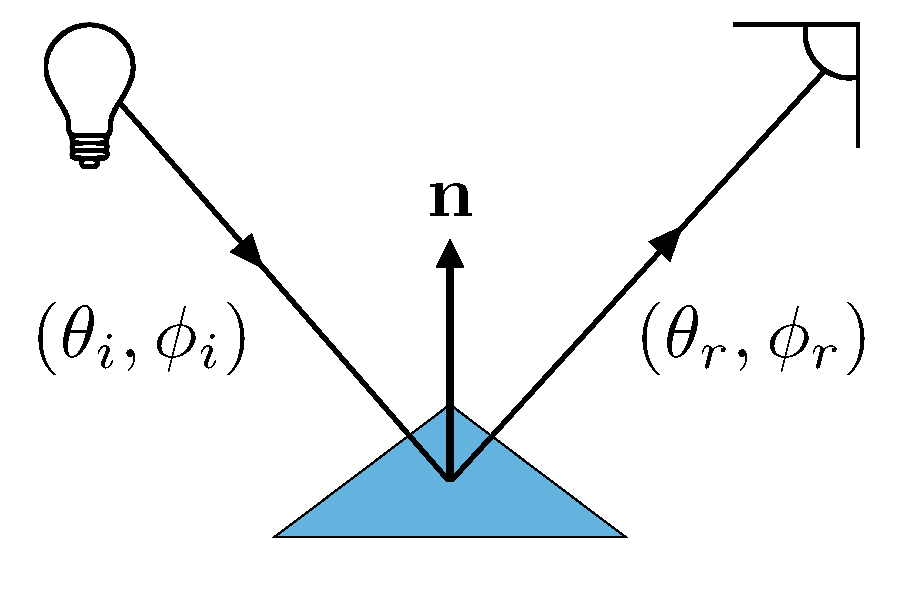
\includegraphics[width=\textwidth]{background/images/general_brdf}
		\caption*{General BRDF}
	\end{subfigure}
	\begin{subfigure}[b]{0.45\textwidth}
		\centering
		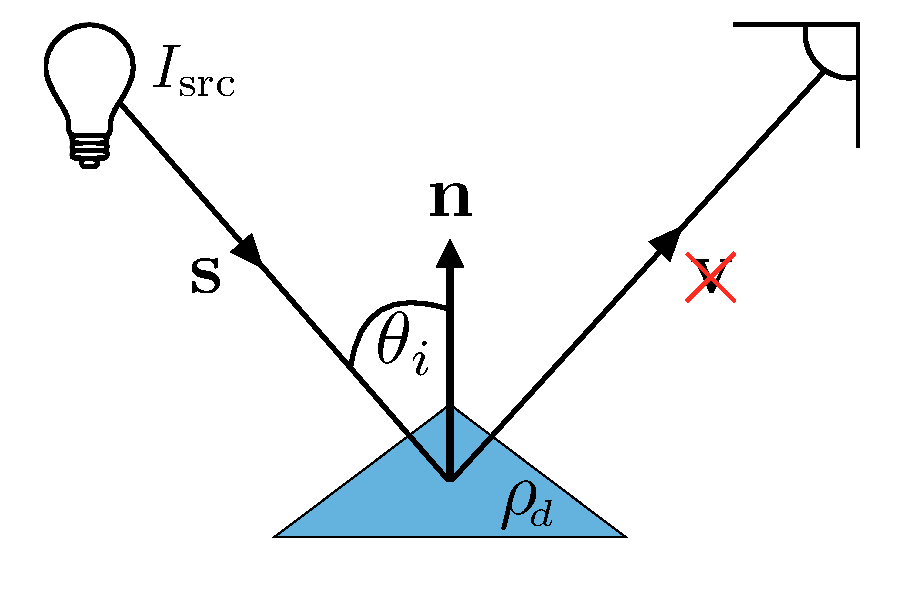
\includegraphics[width=\textwidth]{background/images/lambertian_brdf}
		\caption*{Lambertian BRDF}
	\end{subfigure}
	\caption{The left image shows the general radiance equation for a generic
	         BRDF that is parametrized by the irradiance $(\theta_i, \phi_i)$
	         and radiance $(\theta_r, \theta_r)$ reflecting from the surface.
	         The right image shows the Lambertian BRDF assuming unit light
	         intensity. Note that the Lambertian BRDF is independent of
	         the viewing direction.}
\label{fig:bg_sfs_brdf_example}
\end{figure*}
%%%%%%%%%%%%%%%%%%%%%%%%%%%%%%%%%%%%%%%%

The most commonly assumed BRDF is that of the Lambertian BRDF.\@ A Lambertian
BRDF models only the diffuse component of radiance and is physically accurate
for materials whose reflectance are dominated by scattering effects. For
example, a commonly cited highly Lambertian object is chalk. In more
detail, the Lambertian BRDF modifies \cref{eg:bg_sfs_general_brdf} such that
$f(\theta_i,\theta_r, \Delta \phi) = \rho_{\smallsub{d}} / \pi$ and therefore
the image irradiance is defined as
%%%%%%%%%%%%%%%%%%%
\begin{equation}\label{eg:bg_sfs_lambertian_brdf}
	L_{\operatorname{lambert}} = I_{\operatorname{src}} \frac{\rho_{\smallsub{d}}}{\pi} \cos{\theta_i} =
	I_{\operatorname{src}} \frac{\rho_{\smallsub{d}}}{\pi} \bb{n}^T \bb{s},
\end{equation}
%%%%%%%%%%%%%%%%%%%
where $\bb{n} = {[n_x, n_y, n_z]}^T \in \R^{3}$ is the unit normal of the surface patch,
$\bb{s} = {[s_1, s_2, s_3]}^T \in \R^{3}$ is the unit
light vector and $\rho_{\smallsub{d}}$ is the diffuse albedo scaled by $1/\pi$
to ensure $\rho_{\smallsub{d}} \in [0, 1]$. The Lambertian BRDF is illustrated
in \cref{fig:bg_sfs_brdf_example}. Note that for the Lambertian BRDF, the image
irradiance does not depend on the viewing direction and thus
$L_{\operatorname{lambert}}$ is not a function of $(\theta_r,\phi_r)$.
Physically, this implies that Lambertian surfaces do not exhibit specular
effects and appear evenly lit from all viewing angles, scaled by the cosine
of the angle between the light and normal vectors. Commonly,
\cref{eg:bg_sfs_lambertian_brdf} is simplified further as it is assumed that the
radiant intensity is normalised and thus the most commonly cited form of the
Lambertian BRDF is
%%%%%%%%%%%%%%%%%%%
\begin{equation}\label{eg:bg_sfs_lambertian_simple}
	L_{\operatorname{lambert}} = \rho_{\smallsub{d}} \bb{n}^T \bb{s},
\end{equation}
%%%%%%%%%%%%%%%%%%%
Finally, \cref{eg:bg_sfs_lambertian_simple} may generate outputs that are
not physically realisable. For example, a patch lit from the vector opposite
its normal would produce negative intensity. Therefore, the correct physical
form of the Lambertian BRDF is
$L_{\operatorname{lambert}} = \rho_{\smallsub{d}} \max(\bb{n}^T \bb{s}, 0)$.
For completeness, is it worthwhile noting that the image irradiance, formed
through the interaction of the scene radiance and the optic lens, is not
the final measured pixel intensity value commonly utilized on Computer Vision.
The final measured pixel intensity is a function of the image irradiance
and a non-linear function commonly referred to as the
\textit{camera response function}. The camera response function models a number
of effects such as detector sensitivity, vignetting, lens falloff and the
camera electronics. In fact, many manufacturers intentionally model
the camera response function to simulate the responses of other media
such as film~\cite{grossberg2003space}. The calibration function is consistent
over the entire image area and is invertible. Therefore, the camera response
function modifies the image irradiance as follows: $I = f(L)$ where $I$ denotes
a singe pixel in the image, $f$ denotes the camera response function and $L$
denotes the image irradiance as was being discussed above.
\cref{fig:bg_sfs_scene_to_intensity} gives an illustration of this process. Note
that the transformation from scene radiance to image irradiance is
linear~\cite{horn1979calculating} and was previously ignored when discussing
radiometric terms. Camera response calibration requires acquiring controlled
images of a MacBeth board or other colour chart, or the use of pre-calculated
response model~\cite{grossberg2003space}. Therefore, unless explicitly
mentioned, we make the strong assumption that the camera response function
is the identity function and thus pixels in any given image directly
represent the scene radiance.
%%%%%%%%%%%%%%%%%%%%%%%%%%%%%%%%%%%%%%%%
\begin{figure}[t]
	\centering
	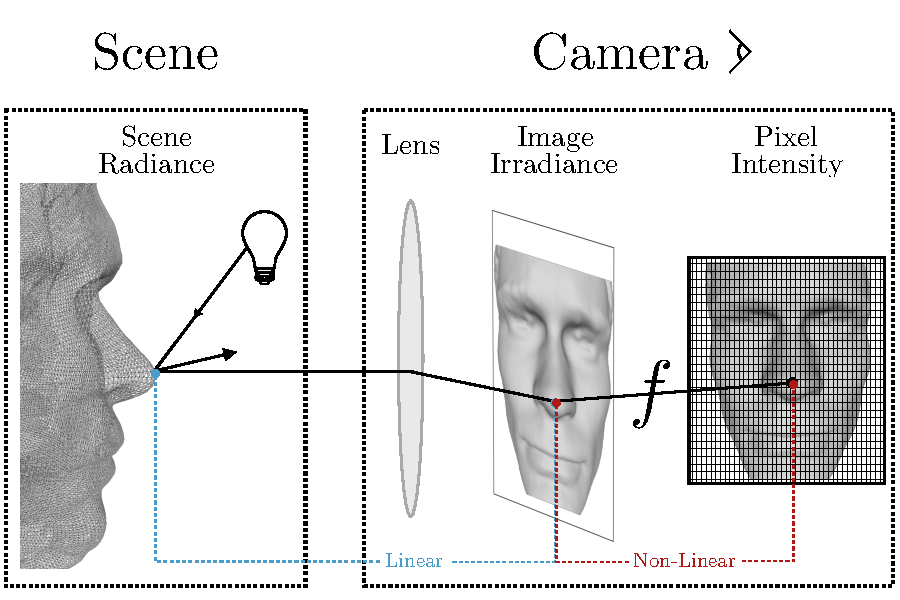
\includegraphics[width=\columnwidth]{background/images/scene_radiance_to_pixel}
	\caption{Illustration of the formation of a pixel intensity in image space
	         from scene radiance. Scene radiance is linearly proportional
	         to image irradiance~\cite{horn1979calculating} and image irradiance
	         is non-linearly mapped to a pixel intensity via the camera
	         response function, $f$.}
\label{fig:bg_sfs_scene_to_intensity}
\end{figure}
%%%%%%%%%%%%%%%%%%%%%%%%%%%%%%%%%%%%%%%%

Even assuming that all of the assumptions outlined above are perfectly
satisfied by an image, SfS is still an under-constrained problem. Given
a single image, $\mathcal{I} \in \R^{w \times h}$ and $d = h \cdot w$, we define
the pixel extraction notation as $\mathcal{I}(x, y)$ which is the scalar
intensity value at the location $(x, y)$ in the image. In the
simple case of an image that depicts a perfectly convex and Lambertian
object with uniform albedo ($\rho_{\smallsub{d}} = 1$), lit by a single
point light of unit flux and known direction that is infinitely far away, the
SfS problem for a single pixel is: $\mathcal{I}(x, y) = {\bb{n}(x, y)}^T \bb{s}$.
Since $\bb{s}$ and $\mathcal{I}(x, y)$ are known, the solution to the problem is a
function of $\bb{n}(x, y)$. An important property of surface normals is that the are
directional vectors that represent local surface orientation. Therefore, they
are parametrised by a unit vector that exists in 3D Cartesian space. However, given the unit norm constraint, surface normals can
also be parametrised as points on the surface of a unit sphere. This is more
evident when normals are converted into spherical coordinates:
%%%%%%%%%%%%%%%%%%%
\begin{equation}\label{eq:bg_sfs_normal_spherical}
    \phi = \arctan{\frac{y}{x}}, \;\;\;\; \theta = \arccos{z}, \;\;\;\; r = 1,
\end{equation}
%%%%%%%%%%%%%%%%%%%
which are clearly a function of two parameters, the azimuth ($\phi$) and
elevation ($\theta$). Similarly, it is common in the SfS literature to
parametrise the surface normals as 2D vectors of the image gradient field:
%%%%%%%%%%%%%%%%%%%
\begin{equation}\label{eq:bg_sfs_normal_pq}
    \bb{n} = \frac{{[p, q, -1]}^T}{\sqrt{p^2 + q^2 + {(-1)}^2}},
\end{equation}
%%%%%%%%%%%%%%%%%%%
where $p = \frac{\partial z}{\partial x}$ and
$q = \frac{\partial z}{\partial y}$ are the parameters of the gradient field
of the surface represented in the image. Therefore, the naive least squares
solution (often termed the \textit{brightness error}) to the SfS problem can be
constructed in matrix form:
%%%%%%%%%%%%%%%%%%%
\begin{equation}\label{eq:bg_sfs_least_squares_lambert}
    \min_{\bb{N}} \lVert \bb{I} - \bb{N} \bb{s} \rVert_F \triangleq
    \min_{\bb{p}, \bb{q}} \lVert \bb{I} - (s_1 \bb{\tilde{p}} + s_2 \bb{\tilde{q}} + s_3 \bb{\tilde{1}}) \rVert_F,
\end{equation}
%%%%%%%%%%%%%%%%%%%
given $d$ is the total number of pixels in the image and
%%%%%%%%%%%%%%%%%%%
\begin{align*}
    \bb{N} &= {[\bb{n}(x_1, y_1), \ldots, \bb{n}(x_w, y_h)]}^T &\in &\R^{d \times 3} \\
	\bb{I} &= {[I(x_1, y_1), \ldots, I(x_w, y_h)]}^T &\in &\R^{d} \\
	\bb{\tilde{p}} &= {\left[\frac{p(x_1, y_1)}{e(x_1, y_1)}, \ldots, \frac{p(x_w, y_h)}{e(x_w, y_h)}\right]}^T &\in &\R^{d} \\
	\bb{\tilde{q}} &= {\left[\frac{q(x_1, y_1)}{e(x_1, y_1)}, \ldots, \frac{q(x_w, y_h)}{e(x_w, y_h)}\right]}^T &\in &\R^{d} \\
 	\bb{\tilde{1}} &= {\left[\frac{1}{e(x_1, y_1)}, \ldots, \frac{1}{e(x_w, y_h)}\right]}^T &\in &\R^{d} \\
	e(x_k, y_k) &= \sqrt{{p(x_k, y_k)}^2 + {q(x_k, y_k)}^2 + 1}. & &
\end{align*}
%%%%%%%%%%%%%%%%%%%
Clearly, this is a function of both $\bb{p}$ and $\bb{q}$ and thus even
the simplest SfS problem is under-constrained. Since
even in the strictest settings SfS is under-constrained, any violations
of the assumptions will only further serve to degrade the recovered shape.

Although surface normals
are a parametrisation of an objects shape, in this thesis we are most
interested in the recovered 3D coordinates. In the case of SfS, this can be
realized as a height map (or depth map) of $z$-coordinates that protrude
from the image plane. Given the $\{p, q\}$ gradient field parametrisation, the
height map may be recovered via integration of the gradient field. However,
due to noise in the gradient field recovery, the gradient field will not be
directly integrable. Therefore, integration of the gradient field into a
surface is itself an area of research. The simplest solution to the
problem is to formulate the integration in terms of the unknown surface,
$\bb{Z}$, and to minimise the least squares error~\cite{horn1990height,simchony1990direct,agrawal2006range}
between the image gradient field and the gradient field of the height map,
$\{\bb{Z}_x, \bb{Z}_y\}$:
%%%%%%%%%%%%%%%%%%%
\begin{equation}\label{eq:bg_sfs_gradient_field_ls}
    \bb{Z} = \int \int {(\bb{Z}_x - \bb{p})}^2 + {(\bb{Z_y} - \bb{q})}^2 \;\; dx dy
\end{equation}
%%%%%%%%%%%%%%%%%%%
which is readily solved via the Poisson equation:
$\nabla^2 \bb{Z} = \operatorname{div}(\bb{p}, \bb{q})$ where
$\operatorname{div}(\bb{p}, \bb{q}) = \frac{\partial p}{\partial x} + \frac{\partial q}{\partial y}$
is the divergence operator. The interested reader should consult the
work of \citet{agrawal2006range}, which provides a unified method for
surface gradient field integration, including the commonly employed Fourier
basis method of \citet{frankot1988method}.

In the following section we review relevant facial SfS algorithms. Unless
explicitly mentioned, the methods below assume that faces exhibit ideal
Lambertian reflectance given by \cref{eg:bg_sfs_lambertian_simple},
which has been shown to be a reasonable approximation
of facial reflectance~\cite{Sirovich:1987te,georghiades2001fromfew,%
Basri:2003ie,turk1991eigenfaces,Hallinan:1994dz,ramamoorthi2002analytic,%
ramamoorthi2001relationship,shashua1997photometric,moses1993face,%
marschner1999image}. For a more
thorough treatment of the generic SfS literature we suggest the surveys
of \citet{zhang1999shape} and \citet{durou2008numerical}.
%%%%%%%%%%%%%%%%%%%%%%%%%%%%%%%%%%%%%%%%%%%%%%%%%%%%%%%%%%%%%%%%%%%%%%%%%%%%%%%%
\subsection{SfS Facial Surface Recovery}
%%%%%%%%%%%%%%%%%%%%%%%%%%%%%%%%%%%%%%%%%%%%%%%%%%%%%%%%%%%%%%%%%%%%%%%%%%%%%%%%
The current state-of-the-art in SfS is the generic method of
\citet{barron2015shape}, called
Shape, Illumination and Reflectance from Shading (SIRFS). The SIRFS method is
described as a generalisation of the modern ``intrinsic image'' algorithm in
which shading is parametrized in terms shape and illumination.
\citet{barron2015shape} seek to recover the most likely explanation, in a
statistical sense, by imposing a set of very general priors around smoothness
and colour composition on the input image. Although this is a state-of-the-art
method, it does not perform well for shape recover of faces.
\citet{li2014intrinsic} extend SIRFS by enforcing facial specific priors. They
use the physically based skin BRDF proposed by \citet{weyrich2006analysis} and
place priors on the skin reflectance parameters using the data
from~\cite{weyrich2006analysis}. They also impose a geometric prior on the face
shape by providing an initial estimate of the 3D face shape
using~\cite{Yang:2011gj}. \citet{li2014intrinsic} show superior results to the
original SIRFS, particular for surface normal recovery.
\citet{atick1996statistical} propose an analysis-by-synthesis method
for minimizing the reconstruction error between a statistical model of facial
surface based on depth images rendered using a Lambertian BRDF and the input
image. Although this is termed as SfS, we classify it as analysis-by-synthesis
and discuss it in further detail in \cref{sec:bg_3dmm}.
\citet{yuan2002sfs} use a neural network in order to constrain the outputs
of a Lambertian SfS algorithm to be in the span of a training set of 3D
depth images.
\citet{fanany2004neural,fanany2002analysis} also propose to use a neural network
for SfM. However, the authors use multiple views of an object and deform
the vertices of a polygonal mesh to be consistent with input from SfS.
\citet{dovgard2004statistical} combine the symmetric SfS method of
\citet{yilmaz2002estimation} with the statistical model of
\citet{atick1996statistical} in order to resolve an ambiguity present in
the symmetric formulation of~\cite{yilmaz2002estimation}.
\citet{smith2010estimating} also use a database of facial surfaces
orthographically projected to form a statistical model of facial shape. They
enforce ``model-based integrability'' by ensuring that normals recovered
by the geometric SfS algorithm of \citet{worthington1999new,Smith:2007eb} lie
in the span of the normals computed from statistical surface model. Furthermore,
\citet{smith2010estimating} show that this framework allows the usage of
more complex BRDFs such as the Phong~\cite{tuong1973illumination} model.
However, although \citet{smith2010estimating} discuss handling non-frontal
illumination, their primary results focus on the case when the illumination
is coincident with the viewing angle.
\citet{biswas2009robust} concentrate on robust albedo estimation, though they
demonstrate the accuracy of their albedo estimation by performing SfS using the
method of \citet{ping1994shape}. In particular, they utilize a mean shape as the
initial shape estimate and thus produce a robust estimate of the albedo using a
Linear Minimum Mean Square Error Estimator (LMMSE). They proceed to normalise
the image using the albedo estimate and then transform the normalised image to
appear lit by the initial illumination direction estimate. Finally, SfS is
performed on the transformed image, which they showed was much more accurate
than performing SfS on the initial input image.
\citet{kemelmacher2011facereconstruction} also utilize a template shape, but
rather than simply initialising a SfS algorithm with this shape, the authors
propose to augment the template geometry with a photometric consistency term
stemming from spherical harmonics. This is similar in spirit to many of the
methods shown in \cref{subsec:bg_capture} where the coarse output of stereo was
augmented with photometric information. 
In \citet{kemelmacher2011facereconstruction} directly optimize over the 3D
surface rather than the normals themselves in order to avoid integration of the
normals as a secondary process. In \citet{kemelmacher2011facereconstruction}, 
the 3D surface is parametrized as a height map and alignment between the input
image and the template mesh is performed via optical flow. This implies that the
method is generally poor at recovering details from posed images as the
alignment between the template and the image must be highly accurate. This work
was also utilized in~\cite{kemelmacher2008mooney} for the recovery of shape
using binary images (dubbed ``Mooney-images'') where the authors show that, with
some consideration, a template mesh may also be deformed to recovery reasonable
facial shape from textureless images.
\citet{roth2015unconstrained} extend the work of~\cite{kemelmacher2011facereconstruction}
by proposing to use a 3D mesh parametrized by vertices rather than as a height
map. 2D facial landmarks are utilized to recover the initial mesh alignment with
the input image and a novel Laplace mesh editing method is used to deform the
template mesh to the photometric normals predicted from the image.
\citet{Suwajanakorn:2014bl} also perturb a template mesh using a photometric
consistency term based on spherical harmonics.
However, \citet{Suwajanakorn:2014bl} deform a person
specific model learnt automatically from Internet images and propose a novel
alignment method they term ``3D-flow''. 3D-flow is an analysis-by-synthesis
method where no statistical constraint is placed on the vertex movements
and thus vertices are free to move in a manner identical to optical flow. In
contrast to other methods described previously, \citet{Suwajanakorn:2014bl}
focus on the recovery of facial shape accurately over sequences.
We note that \citet{nehab2005efficiently} also proposed a general method
for combining coarse templates with normal information.

There are also a number of statistical model based methods that propose the
learning of parametric models of either normals or spherical harmonics.
\citet{smith2006recovering} propose to use a cartographic projection, the
Azimuthal Equidistant Projection (AEP)~\cite{snyder1987map}, to enable
the computation of Principal Component Analysis (PCA) directly on normals. Since
surface normals are vectors it is non-trivial to compute distances between
them. Therefore, the AEP allows PCA to be performed on normals in the tangent
space specified by the projection. Similarly, \citet{smith2008facial} propose
another methodology for computing distances between normals using
Principal Geodesic Analysis (PGA)~\cite{fletcher2004principal}.
Both~\cite{smith2006recovering} and~\cite{smith2008facial} were embedded
in the geometric SfS method of~\cite{worthington1999new} to perform statistical
facial SfS. Similarly, \citet{Ahmad:2011kh} propose to combine the output
from the probabilistic SfS method of \citet{haines2008belief} with the
normals from the statistical model of~\cite{smith2008facial}.
\citet{minsik2009facial} also build a statistical model of surface normals,
but directly on the normals scaled by the albedo, without considering issues
arising from Euclidean distance estimations. PCA is performed on the scaled
normals and then a joint linear model is constructed by weighting the scaled
normals by the lighting coefficients. Several such rotated models are
constructed and at testing time the model with the lowest standard
deviation is chosen to produce the final result. The images are aligned
with an affine alignment using the eye centres and the normals are integrated
using \citet{frankot1988method}.
\cite{minsik2011fast} utilize a tensor decomposition method based on the
2nd order spherical harmonic basis. They compute spherical harmonic
images directly from the surface normals and perform
N-Mode~\cite{vasilescu2003multilinear} on the images of all subjects
to reduce the dimensionality. They then alternately solve for both the
identity mode and the spherical harmonic coefficients to recover the person
specific spherical harmonic images of an input image. Finally, assuming
all images are aligned with an affine alignment, the spherical harmonic
images can be integrated using a method such as~\citet{frankot1988method}.
No further photometric consistency terms are applied.
% TODO: Go through the possible SFS list to see if those citations are
%       relevant or whether they are just relighting papers. At least
%       the tensor splines should be relevant.
%%%%%%%%%%%%%%%%%%%%%%%%%%%%%%%%%%%%%%%%%%%%%%%%%%%%%%%%%%%%%%%%%%%%%%%%%%%%%%%%
